%!TEX root = ./lec03_hardware.tex

%
% ---------------------------------------------------------------------------
%
\begin{frame}{Virtual Memory}
\label{virtual_memory}

Virtual Memory\footnote{\url{https://en.wikipedia.org/wiki/Virtual_memory}} is a powerful programming metaphor that allows the efficient and secure simultaneous execution of multiple programs in the same computer.

\begin{columns}[onlytextwidth]
\begin{column}{0.7\textwidth}

Each program is allowed to use virtually every memory address possible in the computer (e.g., $2^{64}$ addresses in a 64-bit machine).

\vskip0.5em

If the program requires more memory (pages) than is \emph{physically available}, the operating system automatically moves some memory pages to disk, making room for the new requests.

\end{column}
\begin{column}{0.3\textwidth}
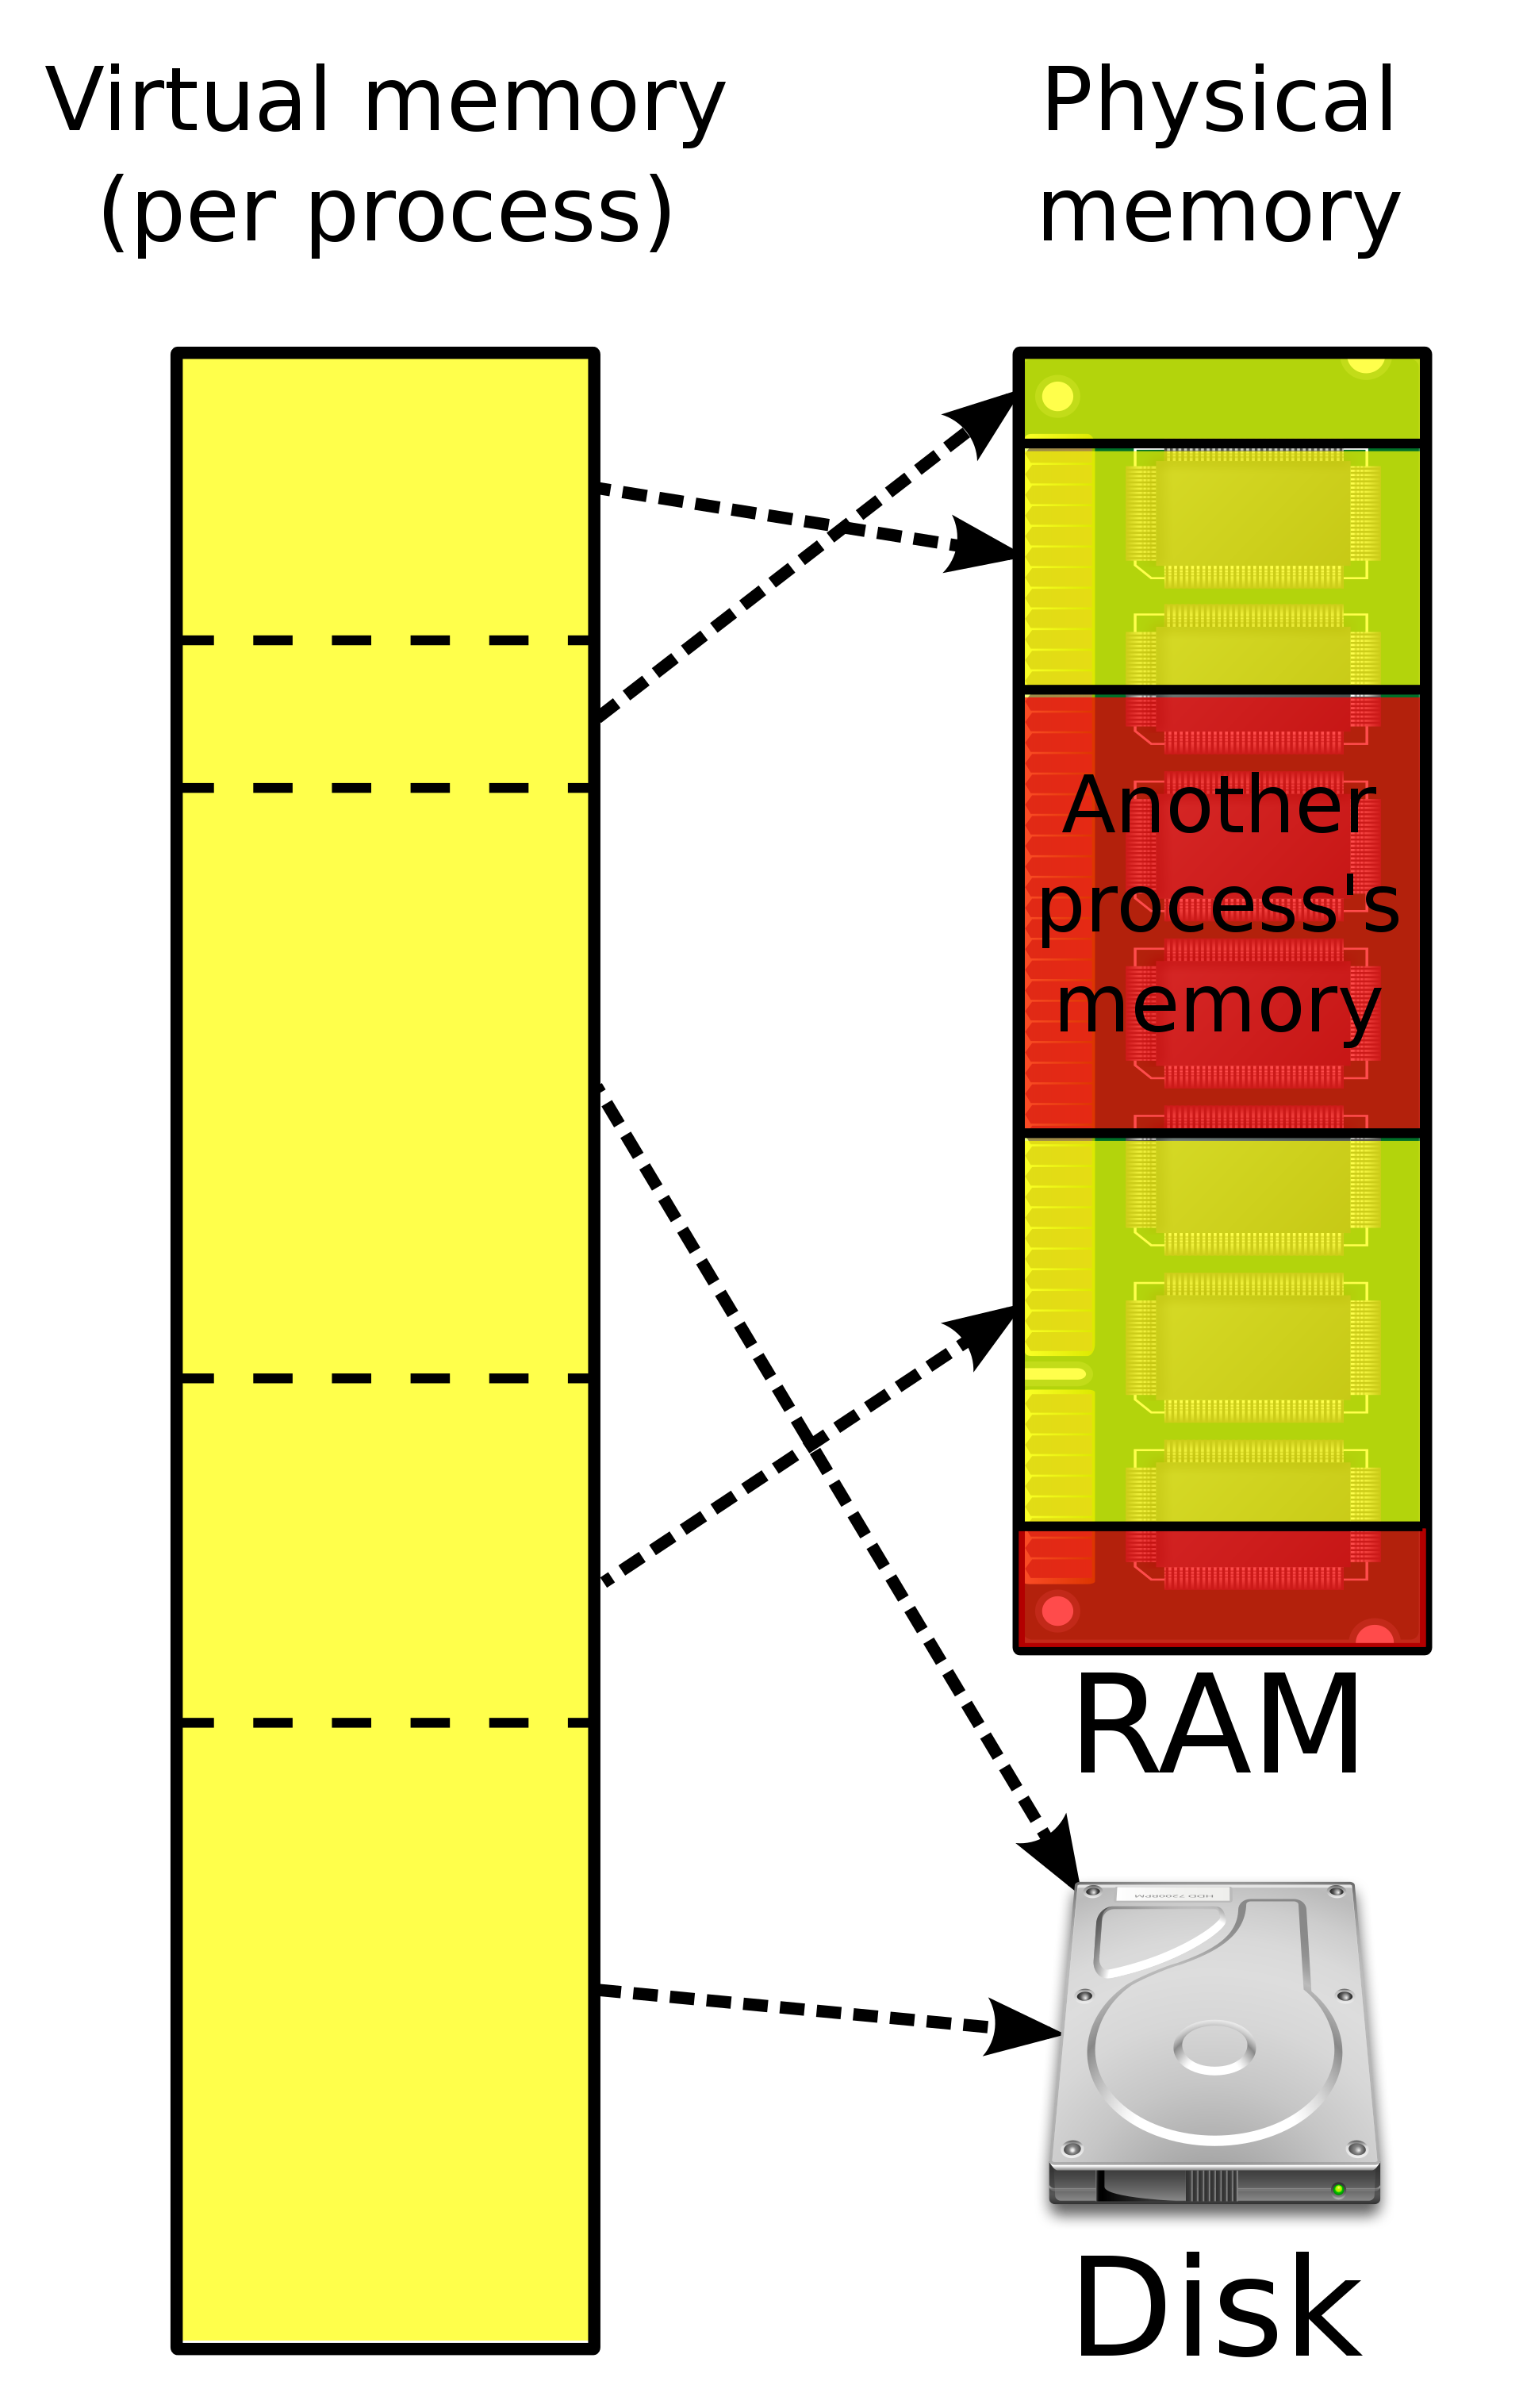
\includegraphics[width=0.9\textwidth]{figures/1920px-Virtual_memory.png}

\hfill{\tiny Source: Wikipedia.}
\end{column}
\end{columns}
\end{frame}


%
% ---------------------------------------------------------------------------
%
\begin{frame}

Programs can use all possible memory addresses (e.g., $2^{64}$ addresses on a 64-bit machine). As a result, virtual memory can have more pages than what is available in physical memory.

\vskip1em

\begin{center}
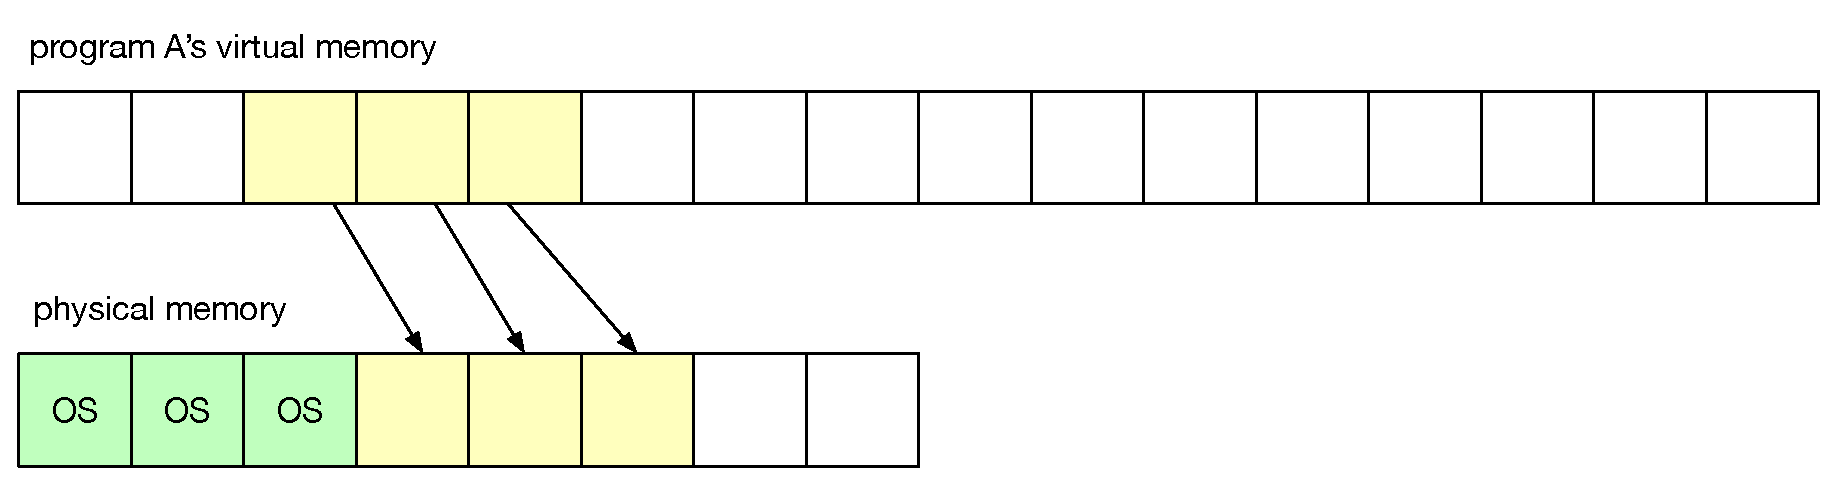
\includegraphics[width=\textwidth]{figures/virtual_memory_scene1.eps}
\end{center}

\vskip1em

As the program requests more memory, the Operating System (OS) assigns physical pages to the virtual pages of the program.

\end{frame}

%
% ---------------------------------------------------------------------------
%

\begin{frame}

Physical memory is shared by all programs in execution, including the OS itself.

\vskip1em

\begin{center}
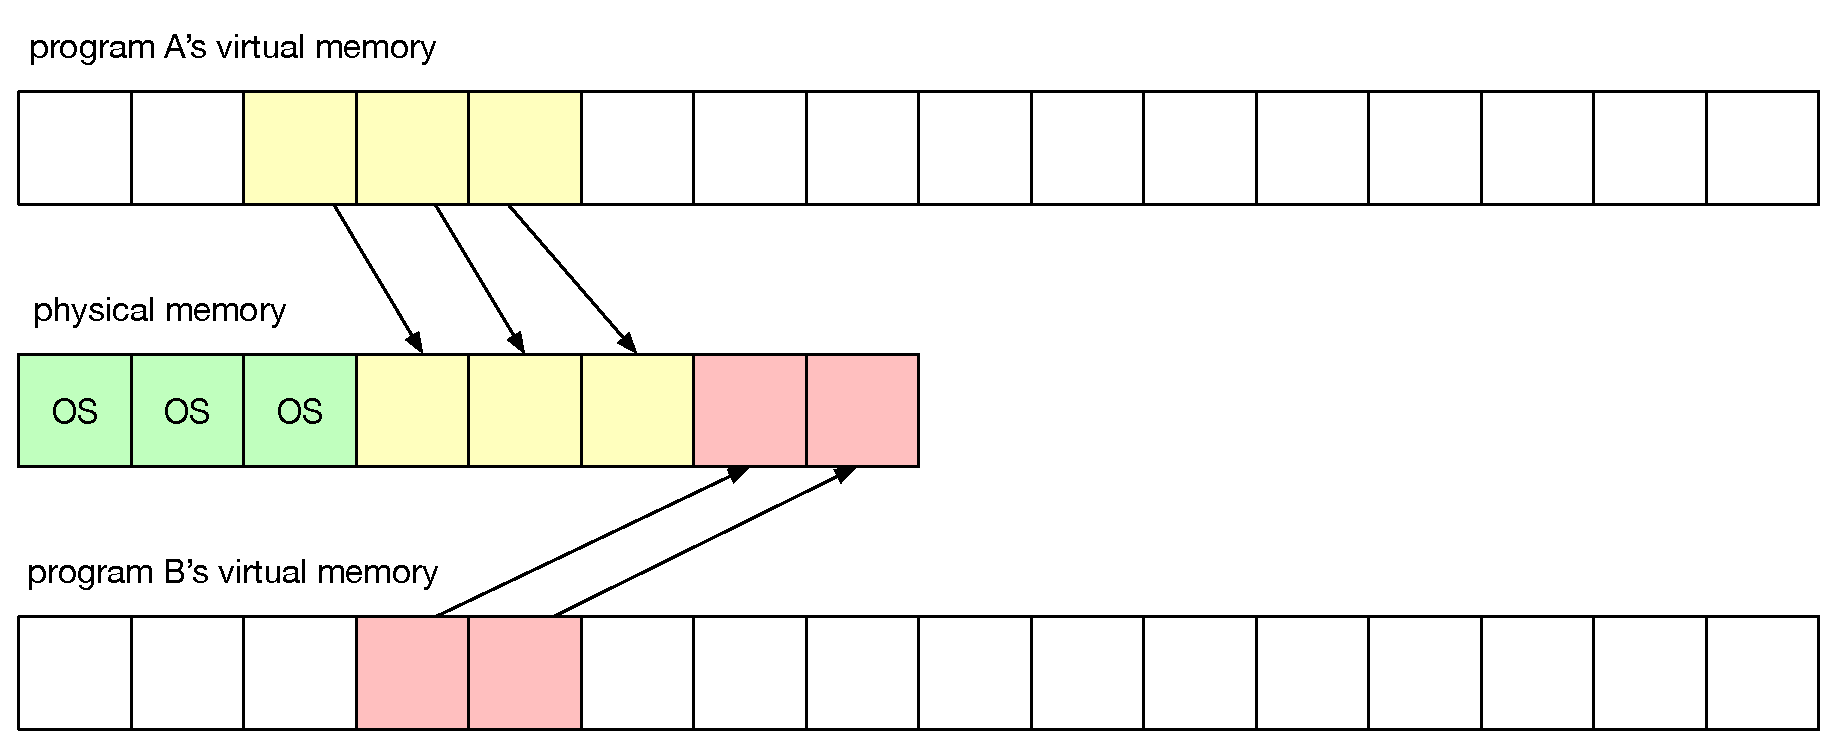
\includegraphics[width=\textwidth]{figures/virtual_memory_scene2.eps}
\end{center}

\vskip1em

Note that two different programs can have pages in the same virtual address, each mapped to a different physical page in main memory.

\end{frame}

%
% ---------------------------------------------------------------------------
%

\begin{frame}

What if a program needs another page but physical memory is full?

\vskip1em

\begin{center}
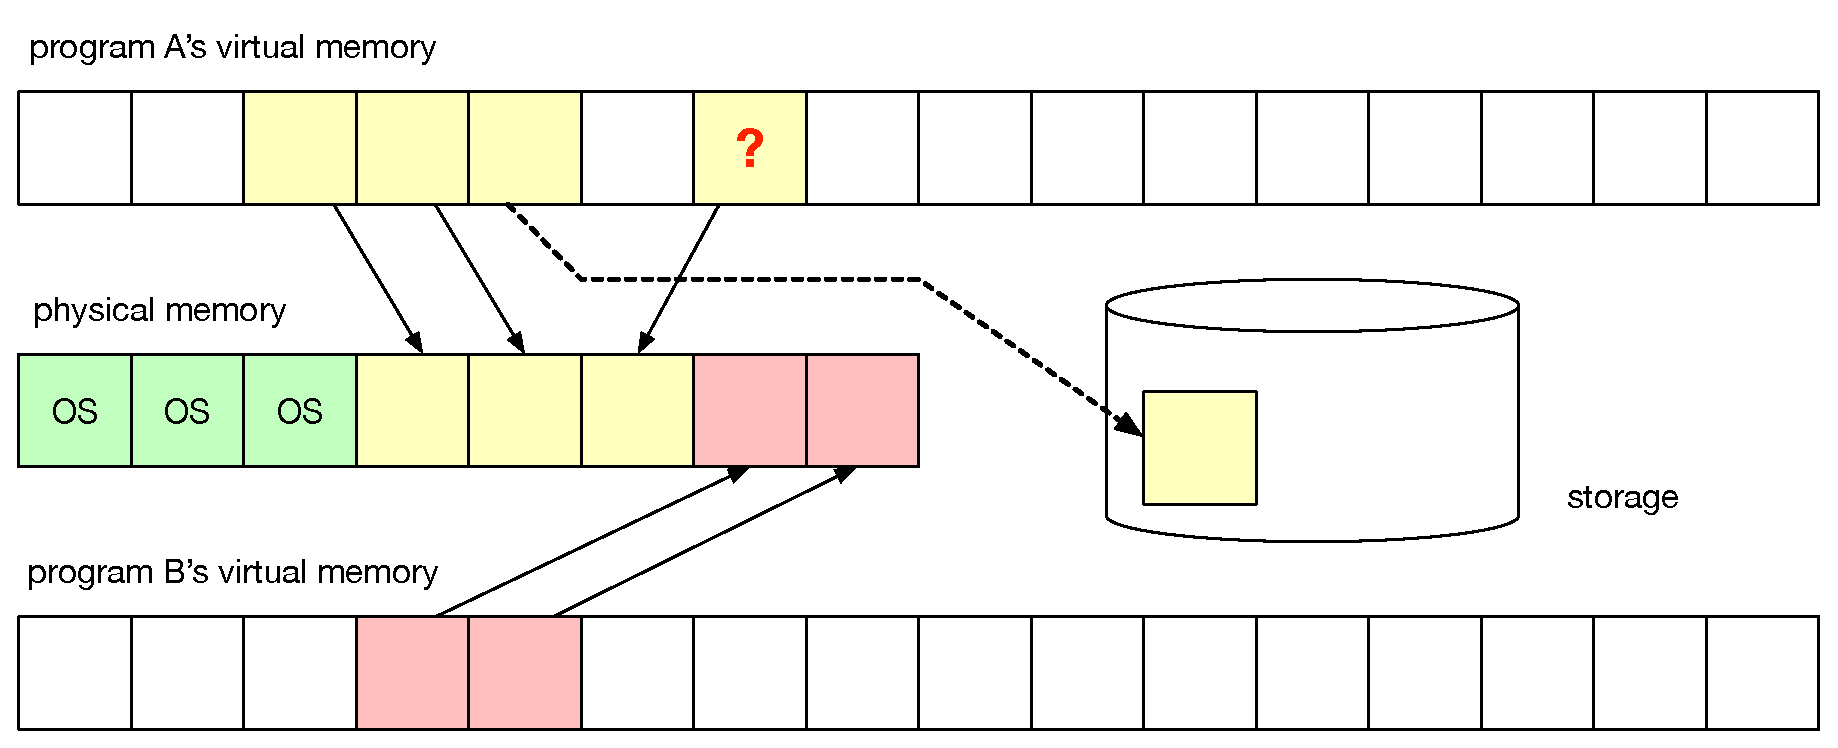
\includegraphics[width=\textwidth]{figures/virtual_memory_scene3.eps}
\end{center}

\vskip1em

The OS takes a page from main memory and \textbf{swaps it out} to storage. This is easy to do because disk blocks and pages have the same size\footnote{Or one is a multiple of the other.}

\end{frame}

%
% ---------------------------------------------------------------------------
%

\begin{frame}

What if a program reads/writes a virtual page that has been swapped out?

\vskip1em

\begin{center}
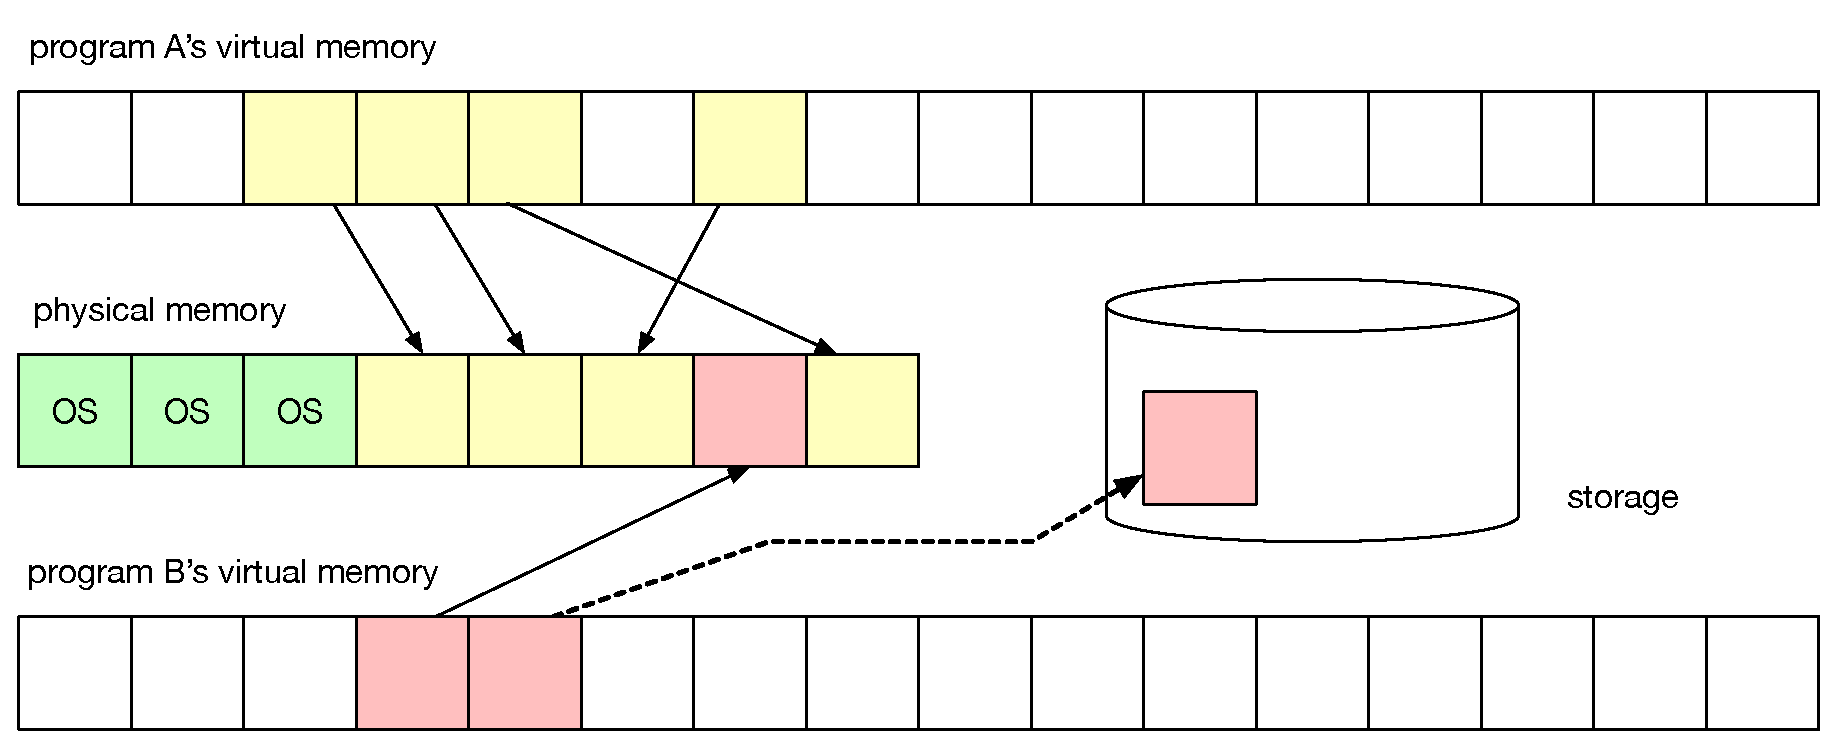
\includegraphics[width=\textwidth]{figures/virtual_memory_scene4.eps}
\end{center}

\vskip1em

The OS takes another page from main memory, \textbf{swaps it out} to storage, making room to \textbf{swap in} the page that was on disk.

\end{frame}


%
% ---------------------------------------------------------------------------
%
\begin{frame}

Recap:
\begin{enumerate}[(1),noitemsep,topsep=-0.5em]
\item Programs always use virtual addresses.
\item The OS places virtual pages into physical pages in memory.
\item The OS moves pages in and out of memory to keep the programs running.
\end{enumerate}

\vskip1em

Recall that memory addresses have 2 parts: $m$ bits for the page, $n$ bits for the offset.

Because virtual and physical pages have the same size, the ``offsets'' in the memory addresses remain unchanged, so all we need to do is to translate ``page'' portion of the address.
\end{frame}

%
% ---------------------------------------------------------------------------
%

\begin{frame}
\label{virtual_memory_size}

The ``size'' of virtual memory in a modern 64-bit CPU is 16 exabytes! No single computer with that much memory exists (and it is unlikely one will ever be built). 

It is common for hardware manufacturers to use fewer bits for physical addresses, based on practical limits.

In any case, the translation of virtual to physical pages considers only the ``page'' part of the address.

\vskip1em

\begin{columns}[onlytextwidth]
\begin{column}{0.6\textwidth}
Example of a modern AMD CPU:

\begin{itemize}[-,noitemsep,topsep=-1em]
\item 64-bit virtual addresses (16 EB)
\item 4KB pages (12 bit offsets)
\item 48-bit real addresses (256 TB\footnotemark)
\end{itemize}
\end{column}
\begin{column}{0.4\textwidth}
\hspace*{-1em}
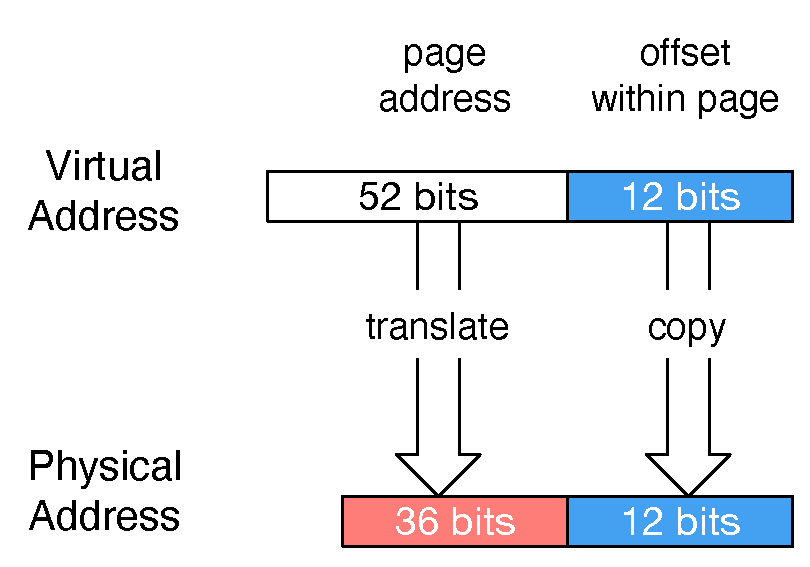
\includegraphics[width=\textwidth]{figures/TLB_translation.eps}
\end{column}
\end{columns}

\footnotetext{Note that this is the maximum allowed.}

\end{frame}

%
% ---------------------------------------------------------------------------
%

\begin{frame}{Implementing Virtual Memory}


Translating virtual page addresses into real page addresses needs to be done fast, and is accomplished with the help of dedicated circuits.

\vskip1em


\begin{BOX}{Virtual Memory Implementation}
\begin{itemize}[-,itemsep=-10pt]
\item the Operating Systems keeps a \textbf{Page Table} mapping virtual pages to real pages;\\

\item the CPU keeps a \emph{cache} of the table in special hardware called \textbf{Translation Lookaside Buffer (TLB)}\\

\item every program has its own page table and TLB entries
\end{itemize}
\end{BOX}

\end{frame}


%
% ---------------------------------------------------------------------------
%
\begin{frame}
\vskip2em
\begin{columns}[onlytextwidth]
\begin{column}{0.4\textwidth}
\textbf{Q:} \alert{\textbf{Which} page(s) should the OS swap out} when needed?

\vskip0.5em

\textbf{A:} Pages that have not been used in a while would be best.

\end{column}
\begin{column}{0.6\textwidth}
\hspace*{1em}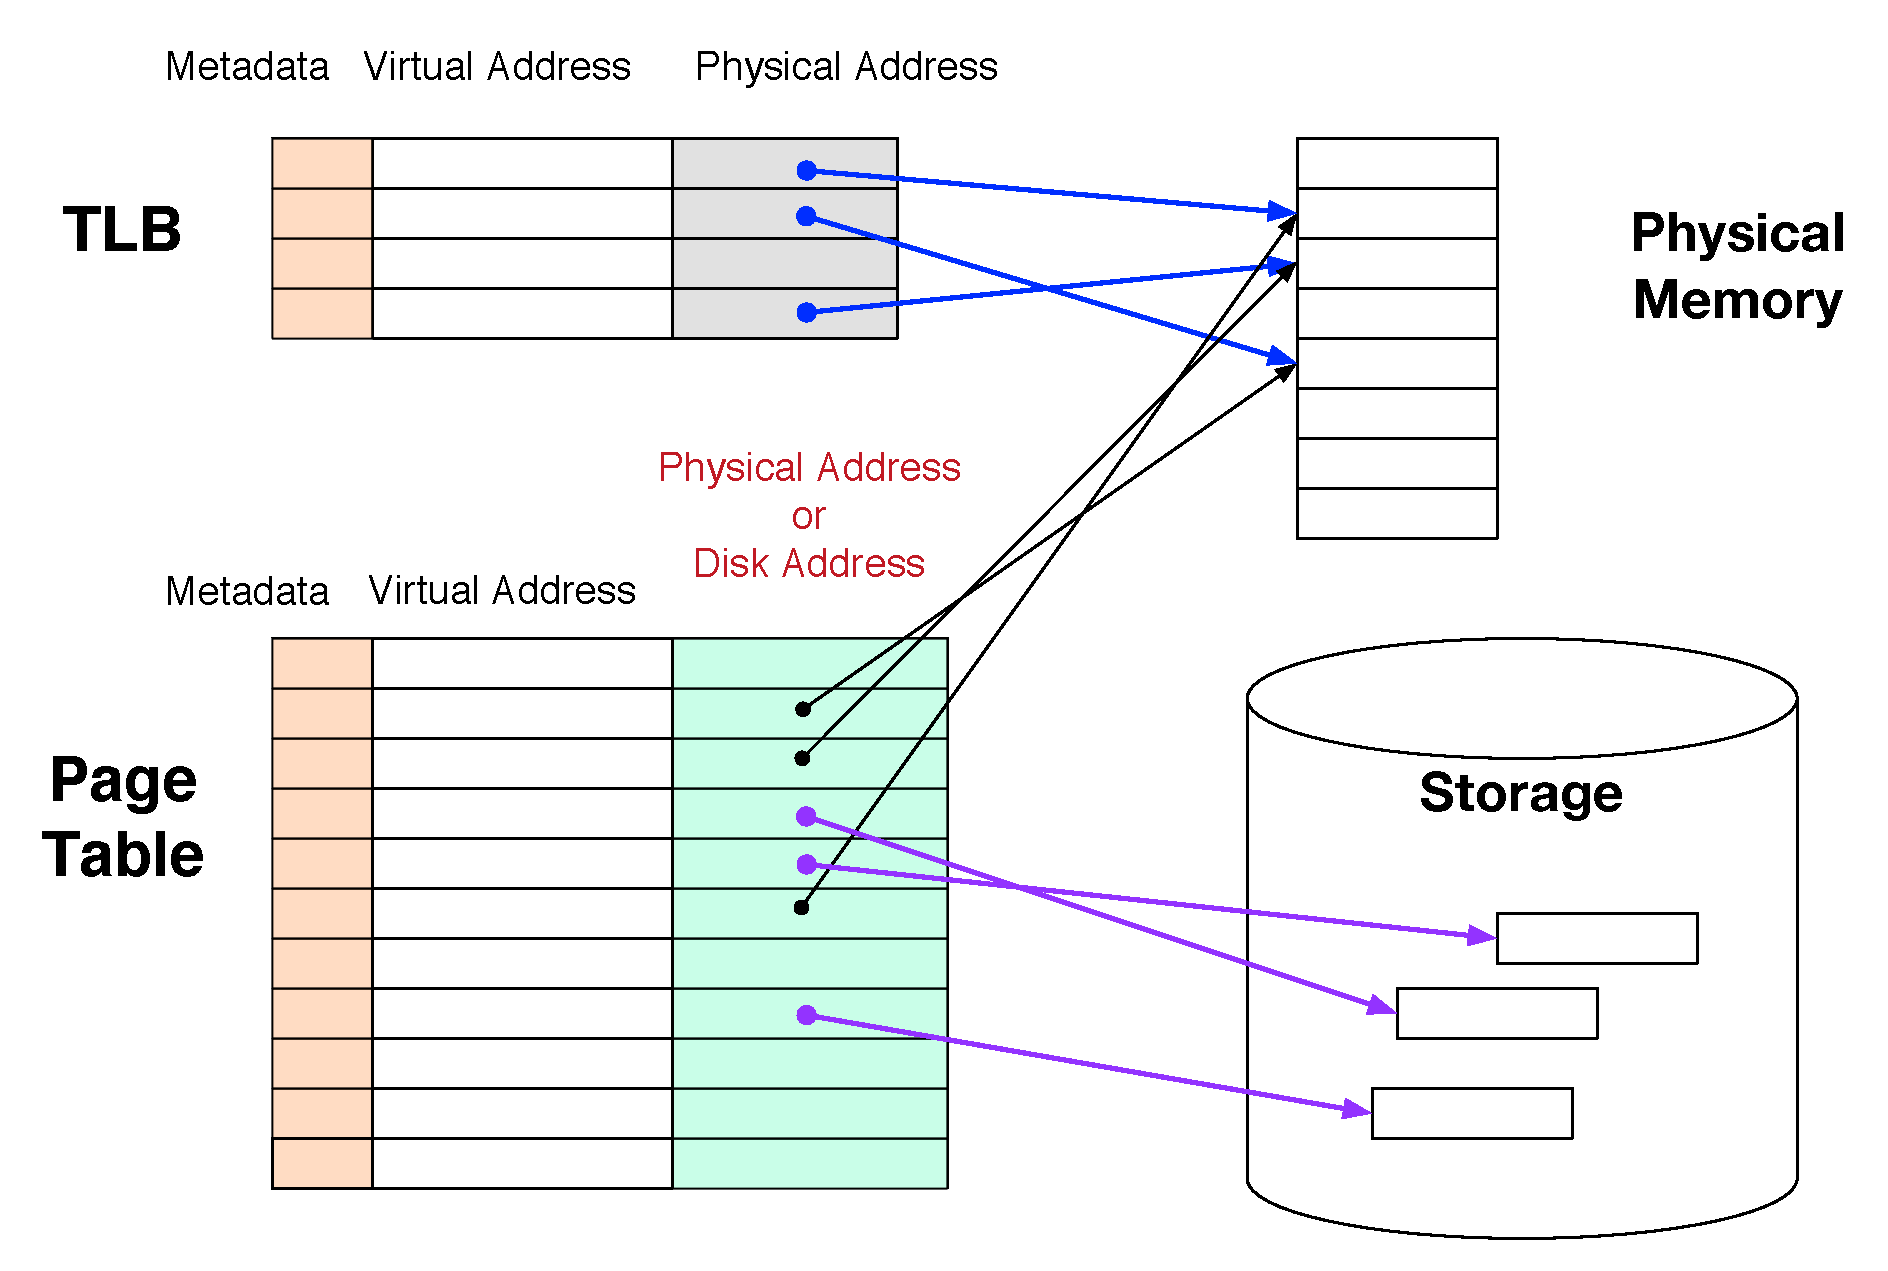
\includegraphics[width=\textwidth]{figures/virtual_memory_TLB.eps}
\end{column}
\end{columns}

\vskip0.5em



The \textbf{metadata} fields in the page table and the TLB keep this kind of information, which the Operating System uses to decide which page to evict.
\end{frame}

%
% ---------------------------------------------------------------------------
%



